\newpage
Un des défis majeurs pour comprendre la régulation de l’expression d’un gène reste encore aujourd’hui de définir quels sont les facteurs qui agissent sur sa transcription. Comme précédemment décrit, les mécanismes de régulation de la transcription des gènes sont nombreux et peuvent agir en cis, sur la même molécule d’ADN, ou en trans par le biais de molécules en circulation dans le noyau (cf Chapitre 1 \ref{chap:regulation-de-expression}). Bien que leur nombre ne soit pas précisément connu, il existe vraisemblablement des centaines de milliers d’éléments \gls{cis}-regulateurs, dépassant très largement le nombre de gènes \citep{encode_project_consortium_integrated_2012}. De nombreuses méthodes permettent de détecter ou prédire la localisation et l’activité des éléments \gls{cis}-régulateurs (cf Chapitre 1 \ref{sec:identif-cis}). Cependant il est encore difficile de définir les gènes cibles de chaque élément \gls{cis}-régulateur. Le rapprochement physique par une boucle de la chromatine est le modèle le plus généralement admis pour expliquer l’activation de l’expression des gènes par les amplificateurs \citep{blackwood_going_1998,bulger_looping_1999, marsman_long_2012}. De nombreux facteurs agissent pour établir de tels repliements, afin de permettre aux amplificateurs de recruter la machinerie de transcription au niveau des promoteurs. La mise en place sélective des paires de promoteur et d’élément \gls{cis}-régulateur pourrait s’effectuer grâce à des modifications précises de la chromatine (ouverture, modifications d’histones, fixation de protéines,...) et par l’action combinée de facteurs agissant en trans se fixant sur les séquences des deux éléments de façon spécifique \citep{ernst_interplay_2013}. La détection et la validation expérimentale de telles paires régulatrices peuvent s’avérer complexes et coûteuses. En effet, observer l’effet d’un éléments \gls{cis}-régulateur sur un gène peut être délicat en raison de la spécificité de la relation (régulation restreinte à un type cellulaire, stade de développement, dépendante de facteurs environnementaux…) ou de nombreux facteurs confondants (redondance fonctionnelle, mécanismes de compensation…). Plusieurs approches d’inférence computationnelle ou expérimentale tentent de prédire les associations entre gènes et éléments \gls{cis}-régulateurs.\\

Au cours de ce chapitre je vais d’abord décrire certaines approches couramment utilisées pour associer les gènes aux élements \gls{cis}-régulateurs. Je m’attacherai ensuite à détailler comment les données expérimentales de contacts de la chromatine seraient en mesure de fournir une description des paysages \gls{cis}-régulateurs. J’effectuerai pour celà une comparaison des paysages \gls{cis}-régulateurs prédits par une approche de voisinage et par les données de contacts de chromatine. Finalement je présenterai un outil que nous avons développé pour inférer les fonctions possibles d’un ensemble d’éléments \gls{cis}-régulateurs selon les gènes qu’ils contactent.

\chapter{Comparaison d'une approche de voisinage et des contacts de la chromatine}
{\hypersetup{linkcolor=GREYDARK}\minitoc}
\label{chap:comp-voisinage}

\section{Prédiction du paysage \textit{cis}-régulateur par une approche de voisinage}
\label{sec:prediction-voisinage}

L’environnement génétique proche a longtemps été un argument majeur pour expliquer les variations de la transcription des gènes. Les premiers modèles qui se sont attachés à expliquer les mécanismes de la régulation ont décrit des séquences promotrices directement en amont des gènes ainsi que des éléments activateurs à seulement quelques dizaines de paires de bases de celles-ci \citep{britten_gene_1969, ptashne_transcriptional_1997}. Les cibles des éléments \gls{cis}-régulateurs ont alors été définies comme étant le ou les gènes les plus proches. Cette approche semble particulièrement justifiée pour les séquences identifiées comme promoteurs des gènes. Pour les éléments \gls{cis}-régulateurs plus distaux, plusieurs études ont confirmé que de nombreux amplificateurs agissent directement sur le niveau d’expression des gènes voisins \citep{banerji_expression_1981, dimattia_pit-1_1997}. De plus, il semblerait que l’action d’une grande majorité des amplificateurs dépend de la distance aux gènes qu’ils régulent. Par exemple, dans une expérience d’intégrations aléatoires de plusieurs gènes \acrshort{GFP} (“Green Fluorescent Protein”) dans le génome de cellules souches de souris, le niveau d’expression de chaque gène de \acrshort{GFP} est négativement corrélé à la distance à l’amplificateur le plus proche \citep{akhtar_chromatin_2013}. Cette même étude estime qu’en moyenne les amplificateurs auraient une influence sur l’expression des gènes autour de 20 kb.\\

L’association des éléments \gls{cis}-régulateurs aux gènes directement voisins s’est généralisée et la grande majorité des études cherchant à inférer des relations régulatrices utilisent une approche de voisinage. Celle-ci présente l’avantage majeur de ne nécessiter aucune donnée moléculaire supplémentaire pour être utilisée. Avec un génome assemblé et annoté en gènes, tout ensemble d’éléments \gls{cis}-régulateurs peut alors être associé facilement à des gènes cibles. L’approche la plus simple consiste à associer les éléments \gls{cis}-régulateurs au gène dont le site d’initiation de la transcription \gls{TSS} est le plus proche dans la limite d’une distance maximale (par exemple 100kb ou 1Mb, Figure \ref{fig:chap2-fig1}.A). Dans d’autres études, un “domaine de régulation” est défini pour chaque gène. Les éléments \gls{cis}-régulateurs s’y trouvant seront attribués à ce gène. Ce domaine de régulation peut être limité jusqu’au \acrshort{TSS} des gènes voisins : un élément \gls{cis}-régulateur sera alors attribué aux deux gènes les plus proches en amont et en aval (Figure \ref{fig:chap2-fig1}.B). Le domaine de régulation peut également se limiter uniquement à une certaine distance et alors être chevauchant pour plus de deux gènes \citep{wong_interplay_2017}. Cette définition est problématique car le choix de la distance maximale a un fort impact sur l'attribution des éléments régulateurs aux gènes. Si elle est faible (5-10kb) une grande proportion d’éléments \gls{cis}-régulateurs n’est associée à aucun gène. Inversement si elle est élevée, de nombreux gènes sont associés à plusieurs centaines d’éléments \gls{cis}-régulateurs ce qui n'est probablement pas réaliste non plus. Une autre approche fréquemment utilisée combine ces deux principes : les frontières des domaines de régulation sont limitées à la fois par une distance maximale et par la présence de \acrshort{TSS} voisin \citep{berthelot_complexity_2018, dukler_phylogenetic_2020}. Une dernière variante consiste à définir un domaine proximal autour du \acrshort{TSS} d’un gène qui sera systématiquement attribué à ce gène indépendamment des gènes voisins et dont la taille sera souvent plus grande en amont (côté promoteur) qu’en aval. Ce domaine proximal est ensuite élargi jusqu’au domaine proximal du \acrshort{TSS} suivant, en respectant également une distance maximale (Figure \ref{fig:chap2-fig1}.C) \citep{berthelot_complexity_2018}. Finalement, dans certaines études, en cas d’incertitude, par exemple si un élément \gls{cis}-régulateur se trouve sur les domaines proximaux de plusieurs gènes, l’association est exclue de l’analyse \citep{dukler_phylogenetic_2020}.\\

\begin{figure}[h]
    \centering
    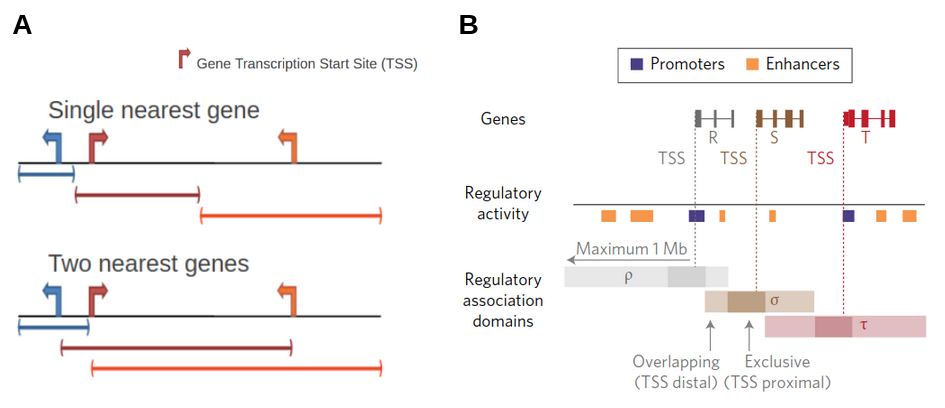
\includegraphics[width=1\textwidth, page=1]{figures/chap2/chap2-fig1.png}
    \caption[Approches d'association entre gène et élément \textit{cis}-régulateur par voisinage.]{
    \textbf{Approches d'association entre gène et élément \textit{cis}-régulateur par voisinage.}
    Pour chaque site d'initiation de la transcription (\acrshort{TSS}), un domaine régulateur est défini de sorte à ce que l'ensemble des éléments \gls{cis}-régulateur y étant inclus lui soit associé.
    \textbf{A.} Approche la plus simple où un élément \gls{cis}-régulateur est associé au \acrshort{TSS} (flèche) le plus proche. Les domaines régulateurs des \acrshort{TSS} (fragments colorés) ne peuvent pas se chevaucher.
    \textbf{B.} Les frontières du domaine régulateur d'un \acrshort{TSS} sont délimitées par les positions des \acrshort{TSS} voisins. Un élément \gls{cis}-régulateur est associé aux deux gènes les plus proches en amont et en aval.
    \textbf{C.} Pour chaque \acrshort{TSS}, un domaine de régulation proximal exclusif est défini, puis étendu jusqu'aux frontières des domaines proximaux des \acrshort{TSS} voisins. Une distance maximale de chaque côté du \acrshort{TSS} peut-être définie, ici 1Mb. A et B sont tirées de l'interface web de GREAT \citep{mclean_great_2010}, C est tiré de \citep{berthelot_complexity_2018}.  \\
    }
    \label{fig:chap2-fig1}
\end{figure} 

Une limitation importante de cette approche est que le nombre d’éléments \gls{cis}-régulateurs attribué à un gène est fortement dépendant de la taille de la région qui le sépare des promoteurs des gènes voisins \citep{taher_variable_2009}. Un gène isolé par de grandes régions intergéniques aura une plus forte probabilité d’être associé avec un nombre élevé d’éléments \gls{cis}-régulateurs. A l’inverse, un gène présent dans une région avec une forte densité de gènes se verra associer un “domaine de régulation” plus restreint. Par exemple, dans le cas des groupements des gènes du développement (tels que les gènes Hox et Evx) bordés par de grandes régions intergéniques souvent nommé "désert de gène”, les gènes situés aux extrémités du groupe pourront être associés avec de très nombreux éléments \gls{cis}-régulateurs \citep{taher_variable_2009}. Cette hétérogénéité de l’organisation des gènes pointe un paramètre confondant important dans la définition des paysages \gls{cis}-régulateurs par une simple approche de voisinage.

\section{Corrélation d’activité entre promoteur et régions régulatrices}
\label{sec:correl-act}

Au cours des 20 dernières années, de nombreux exemples de relations entre gènes et éléments \gls{cis}-régulateurs distaux sont venus défier le modèle d’une régulation exclusivement par voisinage immédiat dans le génome linéaire. Comme évoqué tout au long du chapitre précédent, le gène \gls{SHH} est par exemple régulé par l’amplificateur \acrshort{ZRS} situé dans un intron d’un autre gène à une distance de plus de 800 kb \citep{lettice_long-range_2003}. Un autre exemple est celui de la régulation de l’expression de cinq gènes codants pour plusieurs formes de globulines chez l’humain. Plusieurs amplificateurs situés dans une même région à seulement quelques dizaines de kilobases contrôlent l’expression de ces gènes (Figure \ref{fig:chap2-fig2}) \citep{levings_human_2002}. Selon le tissu et le stade de développement, différents gènes de globulines sont exprimés. Les amplificateurs ne sont alors pas nécessairement associés à l’unique gène le plus proche et peuvent ainsi franchir plusieurs gènes. Selon les modèles d’association par voisinage, un élément \gls{cis}-régulateur est rarement associé à plus de deux gènes (un en amont et un en aval). Dans cet exemple, les amplificateurs auraient été associés au premier gène de e-globuline et à un éventuel gène en amont. De plus, dans les cas de regroupement de gènes, comme celui ci mais aussi dans celui les gènes HoxD contrôlés par la région GCR, plusieurs gènes peuvent être régulés par des éléments \gls{cis}-régulateurs communs \citep{spitz_global_2003}. 

\begin{figure}[h]
    \centering
    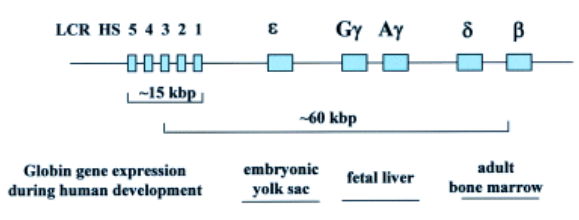
\includegraphics[width=0.8\textwidth, page=1]{figures/chap2/chap2-fig2.png}
    \caption[Schéma de l'organisation génomique des gènes de globulines et de leurs éléments \textit{cis}-régulateurs chez l'humain.]{
    \textbf{Schéma de l'organisation génomique des gènes de globulines et de leurs éléments \textit{cis}-régulateurs chez l'humain.}
    Cinq gènes de globulines sont représentés ainsi que la région LCR ("Locus Control Region") d'environ 15 kilobase contenant cinq éléments \textit{cis}-régulateurs de leur expression. Au cours du développement chez l'humain, le gène e-globuline est exprimé au cours du premier trimestre dans les cellules érythroïdes dérivées de l'hématopoïèse du sac vitellin. Les gènes G-gamma et A-gamma-globulines sont exprimés dans les cellules érythroïdes dans le foie foetal jusqu'à la naissance. Le gène de la bêta-globine est exprimé principalement chez l'adulte dans les cellules dérivées de l'hématopoïèse de la moelle osseuse.
    Les distances ne sont pas à l'échelle. Tiré de \citep{levings_human_2002}\\
    }
    \label{fig:chap2-fig2}
\end{figure} 

L’utilisation des premières données de contact de la chromatine ciblées sur certains loci ont montré que les promoteurs des gènes en interaction physique avec les mêmes régions régulatrices ont tendance à être co-exprimés à travers plusieurs échantillons \citep{dekker_capturing_2002, chepelev_characterization_2012, li_extensive_2012}. Motivé par cette corrélation et surtout par la découverte de la transcription des amplificateurs \citep{kim_widespread_2010}, il a alors été proposé d’utiliser les mesures de l’activité des promoteurs et des amplificateurs pour déterminer leurs associations (cf Chapitre 1 \ref{subsubsec:eRNA}). Par exemple, en utilisant la corrélation de la quantité de transcrits bidirectionnels de chaque paire de promoteur et d’amplificateur à travers plusieurs échantillons, il a été estimé que seuls 40\% des amplificateurs sont associés avec le promoteur le plus proche \citep{andersson_atlas_2014}. Cependant, bien que certaines méthodes existent pour prendre en considération des modèles de co-activité non linéaire \citep{hait_focs_2018}, ces corrélations ne peuvent identifier des interactions régulatrices complexes, par exemple où un gène est régulé par de nombreux amplificateurs optionnels et redondants. Il est également difficile par cette méthode de détecter les paires gène-amplificateur spécifiques d’un type cellulaire, particulièrement lorsqu’un gène est pléiotropique mais qu’une partie de ses éléments \gls{cis}-régulateurs sont spécifiques. Plusieurs autres méthodes de corrélation exploitent l’accumulation des marques de chromatine caractéristiques de l’activité des gènes et des éléments \gls{cis}-régulateurs \citep{whalen_enhancerpromoter_2016, cao_reconstruction_2017}. Celles-ci nécessitent de très nombreuses données pour modéliser et prédire les associations entre gène et amplificateur selon les modifications de la chromatine.  

\section{Mesure des contacts de la chromatine}
\label{sec:mesure-contact}

Les techniques de capture de la conformation de la chromatine permettent de mesurer expérimentalement les contacts (ou la proximité physique) entre des régions du génome. Les premières cartes de contacts de la chromatine à l’échelle du génome complet ont ainsi révélé une structure complexe où de nombreux loci distants se rapprochent spatialement par des boucles d’ADN \citep{schoenfelder_pluripotent_2015, mifsud_mapping_2015}. La vision tridimensionnelle permettrait alors de s’affranchir de la notion de distance linéaire entre les séquences pour déterminer les associations régulatrices. La technique de capture de conformation de la chromatine ciblée sur les promoteurs des gènes (\gls{PCHi-C}, cf Chapitre1 \ref{subsec:HiC}), ouvre aujourd’hui la possibilité de définir plus précisément le paysage \gls{cis}-régulateur de chaque gène. \\

Un de mes premiers objectifs de thèse a été de rassembler l’ensemble des données de \gls{PCHi-C} disponibles à l’échelle génomique. J’ai ainsi récupéré les données brutes de séquençage de 12 publications, recoupant 26 échantillons provenant de 16 types cellulaires pour l’humain \citep{choy_promoter_2018, freire-pritchett_global_2017, javierre_lineage-specific_2016, mifsud_mapping_2015, pan_integration_2018, rubin_lineage-specific_2017}. J’ai ensuite mis en place un traitement bio-informatique pour traiter de façon homogène l’ensemble de ces données pour déterminer les contacts de chromatine. Pour évaluer la présence de contacts potentiellement régulateurs, j’ai utilisé les prédictions d'éléments amplificateurs de l’expression des gènes à partir de différentes sources et types de données \citep{andersson_atlas_2014, roadmap_epigenomics_consortium_integrative_2015, hait_focs_2018}. J’ai effectué des traitements identiques à partir de données de \gls{PCHi-C} et de prédiction d’amplificateurs disponibles pour la souris, que j’utiliserai dans les parties suivantes \citep{comoglio_thrombopoietin_2018, koohy_genome_2018, novo_long-range_2018, schoenfelder_pluripotent_2015, schoenfelder_divergent_2018, siersbaek_dynamic_2017}. Les détails des méthodes employées seront décrits plus amplement dans le Chapitre 3 (cf \ref{chap:chap3}) de cette thèse. Ces méthodes permettent d’obtenir une représentation des contacts de chromatine entre un fragment de restriction couvrant des régions promotrices et d’autres régions du génome qui contiennent potentiellement des éléments \gls{cis}-régulateurs (Figure \ref{fig:chap2-fig3}). De plus, afin d’obtenir un attendu aléatoire des contacts j’ai également produit des simulations pour chaque échantillon, à partir des mêmes fragments de restriction et des mêmes régions promotrices ciblées. Celles-ci tiennent compte du nombre d'interactions par région promotrice, de la distribution des distances (sur le génome linéaire) entre les régions contactées.


\begin{figure}[h]
    \centering
    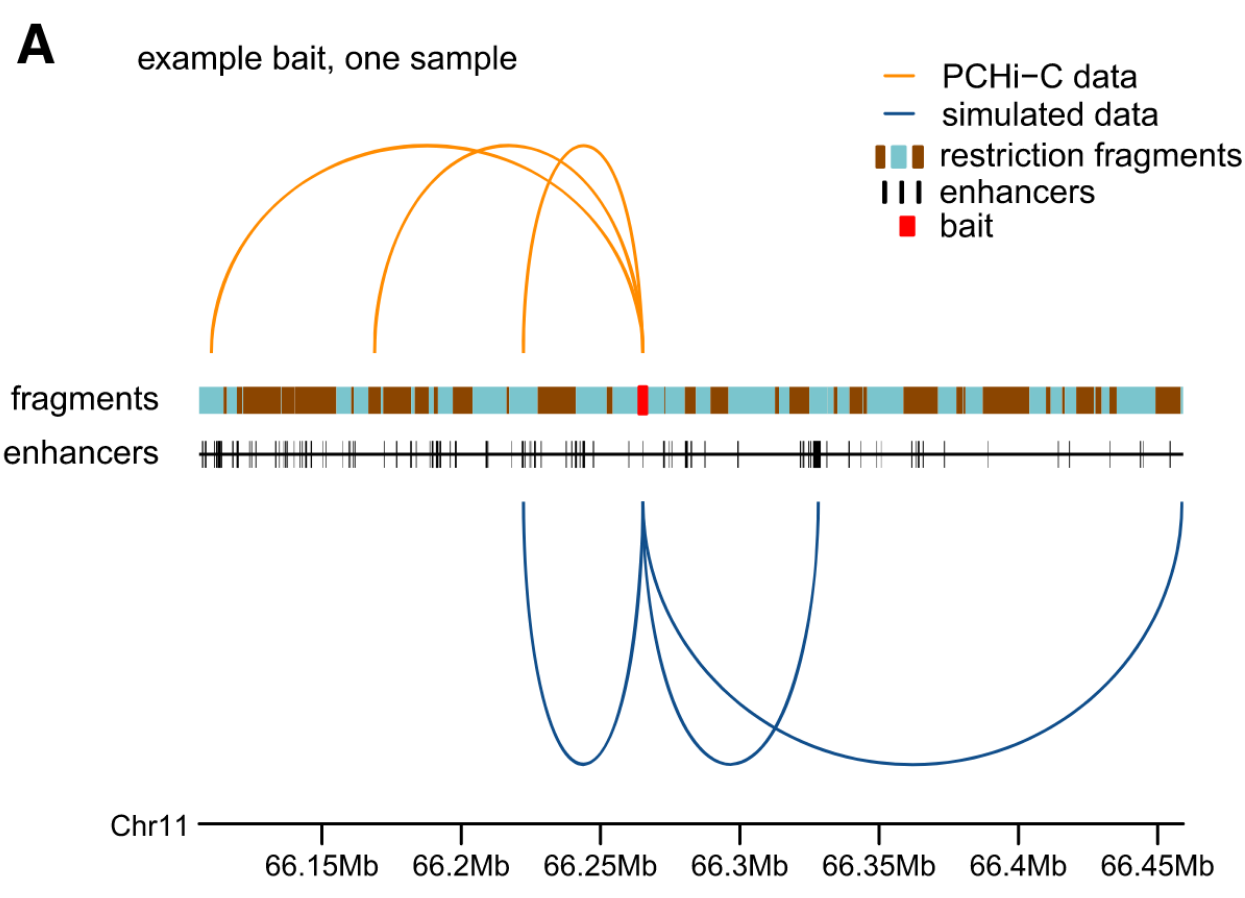
\includegraphics[width=0.8\textwidth, page=1]{figures/chap2/chap2-fig3.png}
    \caption[Contacts de chromatine mesurés par les données de \gls{PCHi-C} et par les données simulée.]{
    \textbf{Contacts de chromatine mesurés par les données de \gls{PCHi-C} et par les données simulée.} Exemple d'interactions entre un fragment de restriction ciblé enrichi en région promotrice (rouge) et d'autres fragments (bleus et marrons), d'après les données de \gls{PCHi-C} (orange) ou les données simulées (bleu). Les positions des amplificateurs ENCODE sont indiquées en noir sous les coordonées des fragments de restrictions. \\
    }
    \label{fig:chap2-fig3}
\end{figure} 

Les premières études utilisant le \gls{PCHi-C} ont montré que les contacts de chromatine sont enrichis en interactions régulatrices. Les régions contactées par les promoteurs sont enrichies en marques d’histones actives (H3K4me1, H3K27ac…) caractéristiques de la présence d’amplificateurs de l’expression \citep{schoenfelder_pluripotent_2015}. Le niveau d’expression des gènes dont les promoteurs sont en contact avec ces régions est corrélé à l’enrichissement de ces marques. De plus, les promoteurs des gènes faiblement ou non exprimés contactent des régions enrichies en marques d’histones répressives (H3K27me3) et pauvres en marques actives. Les gènes contactent ainsi des régions présentant des marques d’histones qui semblent appropriées à leur état d’activité. Les régions contactées sont également enrichies en protéines et facteurs de transcription fixés à la chromatine et associés au niveau d’expression des gènes (RNAPII, CTCF, …) \citep{javierre_lineage-specific_2016}.\\

Nous avons confirmé cet enrichissement en relations régulatrices dans les données combinées de \gls{PCHi-C} (cf Chapitre 3 \ref{chap:chap3})) \citep{laverre_long-range_2022}. Notamment, les régions contactées contiennent une proportion significativement plus grande d’amplificateurs qu’attendu par hasard (Figure \ref{fig:chap2-fig4}.A). La proportion d’amplificateur diminue lorsque la distance aux promoteurs augmente, ce qui pourrait être cohérent avec un modèle de régulation limité à une certaine distance où la majorité des relations régulatrices auraient lieu à proximité des gènes (Figure \ref{fig:chap2-fig4}. C). De plus, nous avons observé une plus grande co-activité des paires gène-amplificateur contactées en \gls{PCHi-C} que dans les données simulées, où la corrélation diminue fortement avec la distance (Figure \ref{fig:chap2-fig4}. B). Les contacts de chromatine mesurés par \gls{PCHi-C} peuvent donc fournir une information pertinente du paysage \gls{cis}-régulateur et permettre une inférence des gènes cibles des éléments \gls{cis}-régulateurs.

\begin{figure}[H]
    \centering
    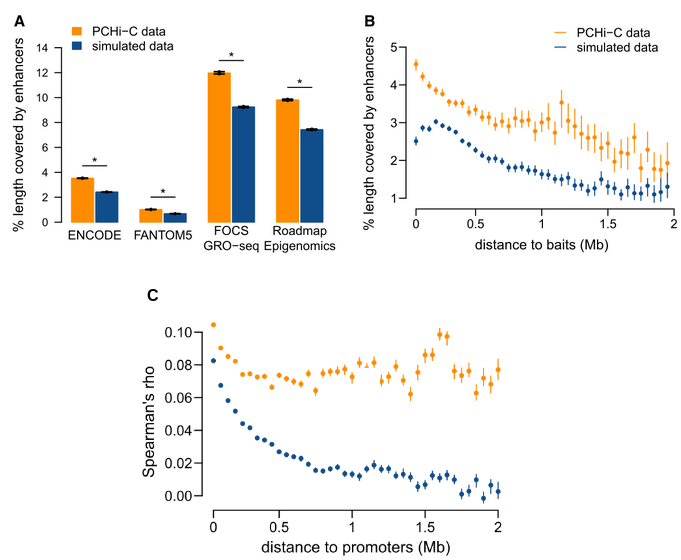
\includegraphics[width=1\textwidth, page=1]{figures/chap2/chap2-fig4.png}
    \caption[Les contacts de chromatine detéctés par \gls{PCHi-C} sont enrichis en relations regulatrices.]{
    \textbf{Les contacts de chromatine detéctés par \gls{PCHi-C} sont enrichis en relations regulatrices.}
    \textbf{A.} Proportion moyenne de la longueur couverte par les amplificateurs prédits par plusieurs méthodes pour les régions génomiques contactées dans les données de \gls{PCHi-C} chez l'humain (orange) et dans les données de contacts simulées (bleu). 
    \textbf{B.} Proportion moyenne de la longeur couverte par des amplificateurs prédits par le consortium ENCODE selon la distance génomique entre les régions promotrices et les régions contactées. 
    \textbf{C.} Distribution des coefficients de Spearman entre les niveaux d'activité des promoteurs et des amplificateurs prédits par ENCODE selon la distance génomique qui les sépare pour les associations déterminées par les données de \gls{PCHi-C} et les données simulées. Les segments verticaux représentent les intervalles de confiance à 95\% de la moyenne. (*) indique une différence significative entre les données de \gls{PCHi-C} et les données simulées (FDR $<$ 10e-10) selon un test de chi2.
    Tirées de \citep{laverre_long-range_2022}.
    }
    \label{fig:chap2-fig4}
\end{figure} 

\section{Comparaison d’une approche de voisinage et des contacts de la chromatine}
\label{sec:comp-voisinage-contact}

L’approche par voisinage étant la plus couramment utilisée, nous avons souhaité comparer les caractéristiques des paysages \gls{cis}-régulateurs des gènes déterminés par celle-ci, par rapport à ceux déterminés par les données de \gls{PCHi-C}. Nous avons ainsi défini un domaine de régulation pour chaque gène délimité par les \acrshort{TSS} des gènes voisins les plus proches en amont et en aval. Chaque amplificateur situé dans cette zone a été attribué au gène. Dans les deux approches, nous avons considéré uniquement les amplificateurs situés à une distance maximale de 2Mb du \acrshort{TSS} des gènes codants pour des protéines. Tous les gènes ne sont pas représentés dans les données de \gls{PCHi-C} car seules certaines régions promotrices sont ciblées par le protocole expérimental. Elles contiennent 70\% (15,702 sur 22,686) des \acrshort{TSS} de gènes codants pour des protéines chez l’humain. 

\subsection{Complexité des paysages \textit{cis}-régulateurs prédits}
\label{subsec:complexité-predit}

Dans un premier temps nous avons analysé les différences de complexité, définie par le nombre d’amplificateurs, des paysages \gls{cis}-régulateurs des gènes dans chacune des approches. Le nombre d’amplificateurs attribué aux gènes est plus grand dans les données de \textbf{contact de chromatine} (médiane = 17) que par une association par \textbf{voisinage} (médiane = 11) (Figure \ref{fig:chap2-fig5}.A). Pour les gènes associés à au moins un amplificateur par les deux approches (N=12,553), les différences du nombre d’amplificateur sont très variables mais l’approche par \gls{PCHi-C} attribue en moyenne plus d’amplificateur par gène (Figure \ref{fig:chap2-fig5}.C, différence moyenne = 6.89). De plus, les complexités des paysages \gls{cis}-régulateurs évalués avec les deux méthodes sont faiblement corrélées (rho de Spearman=0.18; p-value $<$ 2.2e-16). Les données de \textbf{\gls{PCHi-C}} prédisent ainsi un nombre plus important de paires gène-amplificateur (425,168) que l’approche par \textbf{voisinage} (338,644). Comme attendu, ces paires franchissent des distances génomiques significativement plus grandes dans les données \gls{PCHi-C} (médiane = 269 kb) qu’avec une approche de voisinage (médiane = 49 kb; test de Wilcoxon p-value $<$10e-10) (Figure \ref{fig:chap2-fig5}.B). Ceci s’explique en partie par le fait que les contacts de chromatine entre des régions séparées par une distance de moins de 25 kb sont exclus de l’analyse en \gls{PCHi-C}, là où sont présentes 34\% des paires prédites par voisinage. En effet, en raison de la plus grande probabilité d’observer des régions en proximité physique dans le noyau lorsque celles-ci sont voisines sur le génome linéaire, il est difficile d’estimer avec fiabilité la proportion de contacts régulateurs à moins de 25 kb \citep{cairns_chicago_2016}. Dans l’intervalle de distance 25 kb-2 Mb, 43,940 paires gène-amplificateur sont prédites en commun par les deux approches. Du point de vue des contacts \textbf{\gls{PCHi-C}}, ces paires communes sont majoritairement celles séparées par une courte distance génomique (37\% de paires en commun entre 25 et 75 kb) et cette proportion diminue très rapidement pour être inférieure à 5\% à partir de 250kb. Du point de vue des paires gène-amplificateur définies par le \textbf{voisinage}, on observe une diminution de paires en commun avec la distance, mais on note une augmentation pour les distances les plus grandes. Les paires prédites par \textbf{voisinage} à plus de 1Mb sont composées de gènes séparés par de très grandes régions intergéniques.\\

\begin{figure}[H]
    \centering
    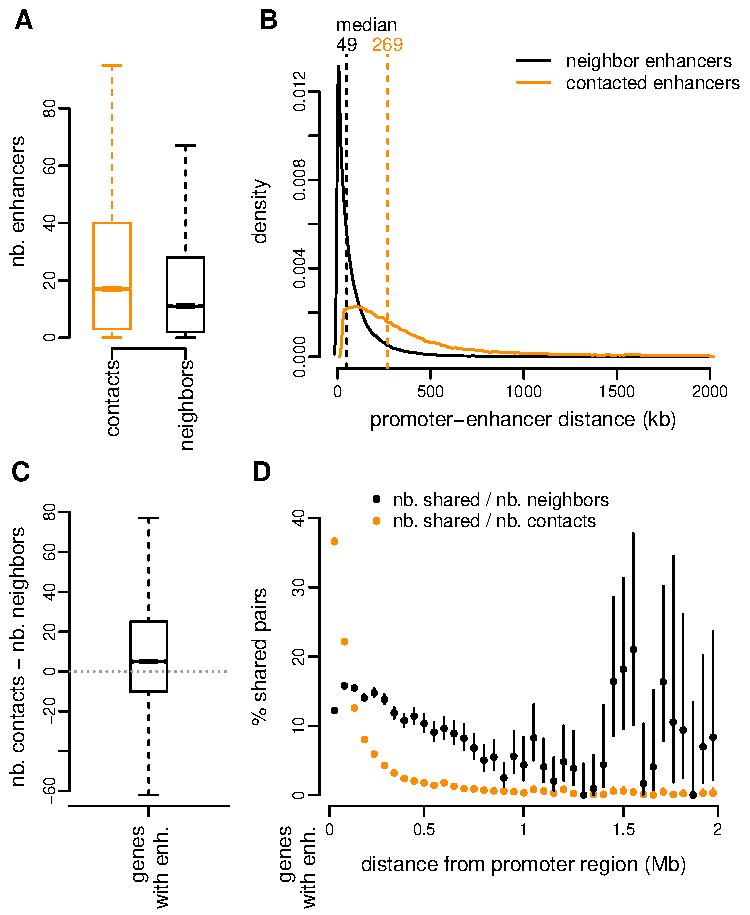
\includegraphics[width=0.7\textwidth, page=1]{figures/chap2/chap2-fig5.pdf}
    \caption[Comparaisons des associations entre gène et amplificateurs inférées par les données de \gls{PCHi-C} et par une approche de voisinage.]{
    \textbf{Comparaisons des associations entre gène et amplificateurs inférées par les données de \gls{PCHi-C} (orange) et par une approche de voisinage (noir).}
    \textbf{A.} Distributions du nombre d'amplificateurs attribués à chaque gène avec les données \gls{PCHi-C} ou avec l'approche de voisinage.
    \textbf{B.} Densité de la distribution des distances génomique entre les promoteurs des gènes et les amplificateurs, pour les deux approches. 
    \textbf{C.} Distribution de la différence du nombre d'amplificateurs attribués à chaque gène avec l'approche \gls{PCHi-C} et l'approche de voisinage. 
    \textbf{D.} Pourcentage de paires gène-amplificateur partagées entre les deux approches, en fonction de la distance génomique entre les promoteurs et les amplificateurs.
    }
    \label{fig:chap2-fig5}
\end{figure} 

\subsection{Taille des domaines de régulation}
\label{subsec:taille-domaine}

Nous avons ensuite évalué la relation entre la taille du domaine de régulation et la complexité des paysages \gls{cis}-régulateurs. Pour l’approche de \textbf{voisinage}, la taille du domaine de régulation, qui est majoritairement déterminée par la distance aux \acrshort{TSS} voisins, est corrélée positivement au nombre d’amplificateurs qui lui sont attribués (Figure \ref{fig:chap2-fig6}.A; rho de Spearman=0.73 ; p-value $<$ 2.2e-16). Les gènes associés à de nombreux amplificateurs voisins sont enrichis pour des fonctions associées à des processus du développement (Figure \ref{fig:chap2-fig6}.B). La taille du domaine défini pour l'approche de \textbf{voisinage} est peu corrélée au nombre d’amplificateurs associés aux gènes par \gls{PCHi-C}, qui reste en moyenne à 15 amplificateurs par gène (rho de Spearman= -0.04; p-value $<$ 6.1e-6). Par contre, la taille du domaine de contact d’un gène définie par la somme des longueurs des régions contactées en \gls{PCHi-C}, est fortement corrélée avec le nombre d’amplificateurs qui lui sont attribués (rho de Spearman= 0.72 ; p-value $<$ 2.2e-16). Il est intéressant de noter qu’il n'existe qu’une faible corrélation entre la taille du domaine \textbf{voisin} et la taille du domaine \textbf{contacté} (rho de Spearman= 0.04 ; p-value $<$ 1.1e-5). Ceci indique notamment que le nombre d’amplificateur associé à un gène dépend du nombre et de la taille des régions \textbf{contactées} mais pas du \textbf{voisinage} du gène. Les gènes associés à de nombreux amplificateurs selon les données de PCHi-C sont enrichis en fonctions de régulation de processus métabolique (Figure \ref{fig:chap2-fig6}.C).

\begin{figure}[H]
    \centering
    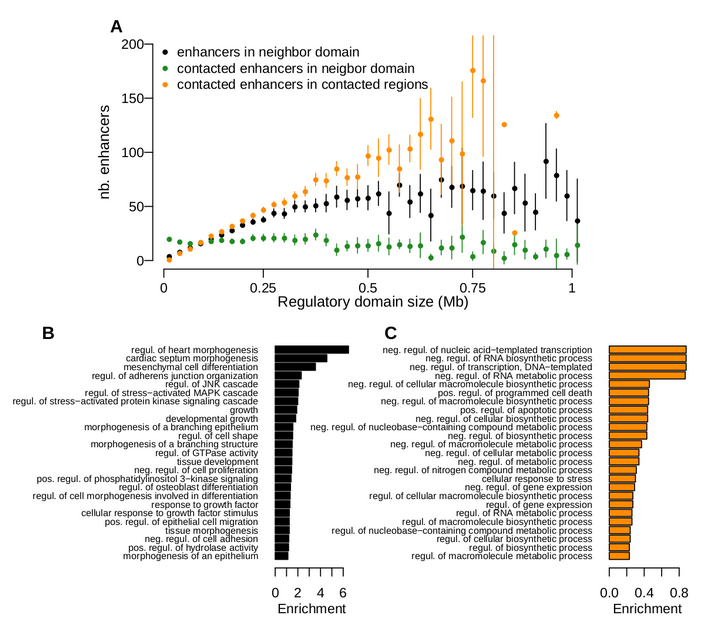
\includegraphics[width=0.9\textwidth, page=1]{figures/chap2/chap2-fig6.png}
    \caption[Attribution des amplificateurs aux gènes cibles selon les domaines de régulation.]{
    \textbf{Attribution des amplificateurs aux gènes cibles selon les domaine de régulation.}.
    \textbf{A.} Nombre moyen d'amplificateur attribué aux gènes selon la taille du domaine régulateur défini par une approche de voisinage (noir) ou par les contacts de chromatine mesurés par \gls{PCHi-C} (orange). Le nombre moyen  d'amplificateur contacté par les gènes en \gls{PCHi-C} et à la fois présent dans les domaines régulateurs défini par voisinage est representé en vert. 
    \textbf{B.} Enrichissement ontologique des gènes triés par ordre décroissant du nombre d'amplificateur leur étant attribué par l'approche de voisinage. Seuls les 25 termes les plus enrichis sont montrés (FDR $<$ 10e-5).
    \textbf{C.} Idem que B. pour les amplificateurs attribués dans les données de \gls{PCHi-C}.
    }
    \label{fig:chap2-fig6}
\end{figure}

\subsection{Relation entre nombre d’amplificateur et expression des gènes}
\label{subsec:complexite-expression}

Nous avons ensuite évalué la relation entre les paysages \gls{cis}-régulateur prédits par les deux approches et le patron d’expression des gènes dans plusieurs organes et stades de développement \citep{cardoso-moreira_gene_2019}. Nous avons mesuré le niveau moyen d’expression des gènes ainsi que l’étendue de l’expression d’un gène, une mesure du nombre d'échantillons dans lequel le gène est exprimé \citep{laverre_long-range_2022}. Nous confirmons que le niveau d’expression des gènes est positivement associé avec le nombre d’amplificateurs \textbf{contactés} dans les données de \gls{PCHi-C} (Figure \ref{fig:chap2-fig7}. A; test de Kruskal–Wallis, p-value $<$ 10-10) \citep{javierre_lineage-specific_2016}. Ceci est en accord avec le rôle activateur de l’expression des amplificateurs avec un effet additif important \citep{schoenfelder_pluripotent_2015, mifsud_mapping_2015}. On observe aussi une forte relation entre le nombre d’amplificateurs \textbf{contactés} et l’étendue de l’expression des gènes (Figure \ref{fig:chap2-fig7}.B; test de Kruskal–Wallis, p-value $<$ 10-10). Plus un gène possède d’amplificateurs et plus celui-ci est actif dans un grand nombre d'échantillons, ce qui ne semble pas être le cas pour le nombre d’amplificateurs \textbf{voisins}. Cependant, contrairement à certaines études nous n’observons pas de relation entre l’expression des gènes et le nombre d’amplificateurs \textbf{voisins}. Cette différence peut s’expliquer par le fait que nous ne tenons pas compte de l’activité des amplificateurs au sein de chaque échantillon dans aucune des deux approches. En considérant seulement les amplificateurs \textbf{voisins} actifs dans le même tissu où l’expression des gènes est mesurée, l’estimation de l’ensemble du paysage \gls{cis}-régulateur d’un gène permet d’observer une relation avec le niveau d’expression \citep{berthelot_complexity_2018}.\\

\begin{figure}[h]
    \centering
    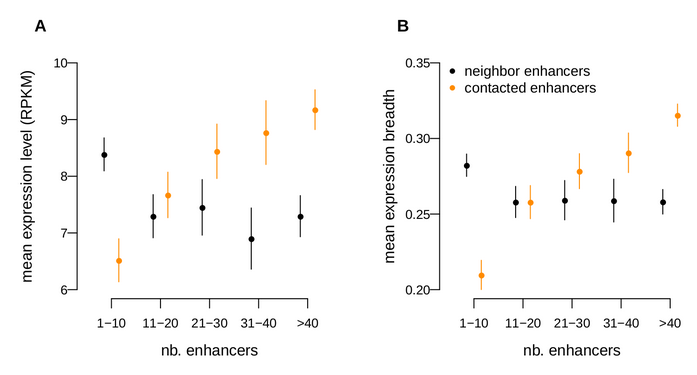
\includegraphics[width=0.8\textwidth, page=1]{figures/chap2/chap2-fig7.png}
    \caption[Relations entre le nombre d'amplificateurs et l'expression des gènes.]{
    \textbf{Relations entre le nombre d'amplificateurs et l'expression des gènes}. Les amplificateurs sont attribués aux gènes selon une approche de voisinage (noir) ou selon les données de contact de chromatine identifés par \gls{PCHi-C} (orange).
    \textbf{A.} Niveau moyen d'expression des gènes selon le nombre d'amplificateur attribués.
    \textbf{B.} Etendue du niveau de l'expression selon le nombre d'amplificateur.
    L'expression des gènes est mesurée sur plusieurs organes et stades de développement d'après les données de \citep{cardoso-moreira_gene_2019} (cf Méthodes dans la Partie \ref{part:chap3}).
    }
    \label{fig:chap2-fig7}
\end{figure} 

Bien qu’il s’intersectent dans une certaine mesure, les paysages \gls{cis}-régulateurs des gènes sont ainsi très différents lorsqu’ils sont définis selon une approche d’association par voisinage ou par les données de contact de chromatine. Le nombre absolu d’amplificateurs par gène n’est pas fortement corrélé entre les méthodes et ceux-ci sont surtout situés à des distances génomiques très différentes par rapport aux promoteurs. Les gènes auxquels on attribue de nombreux amplificateurs sont très différents selon les approches. Cette comparaison a confirmé que les contacts de chromatine ne mettent généralement pas en interaction les gènes et les amplificateurs directement voisins. La distance entre les \acrshort{TSS} voisins (qui dépend de la taille des régions intergéniques ainsi que de la longueur totale des gènes) est le facteur principal de la complexité du paysage \gls{cis}-régulateur d’un gène par l’approche de voisinage. L’organisation du génome est donc un facteur majeur dans l’attribution des éléments \gls{cis}-régulateurs aux gènes avec cette approche. Les contacts de chromatine semblent quant à eux être indépendants de l’organisation génomique unidimensionnelle, c’est-à-dire de la répartition des gènes sur le génome linéaire. Il existe des biais dans les deux méthodes, qui peuvent aller dans des directions opposées. Par exemple, l’approche par \gls{PCHi-C} n’est pas en capacité d’inférer des interactions à très courtes distances (inférieure à 25kb) qui pourraient avoir une grande importance fonctionnelle. De plus, elle ne permet pas de distinguer avec précision les relations régulatrices entre des contacts mettant en relation des régions contenant plusieurs promoteurs ou amplificateurs proches. Ces observations soulignent la complexité de la définition des paysages \gls{cis}-régulateurs de l’expression des gènes. Aucune approche ne semble parfaite mais les données de contacts de la chromatine peuvent permettre d’apporter un nouveau regard sur les relations régulatrices et aider à mieux comprendre les déterminants génétiques de l’expression des gènes. 


\section{Inférer les fonctions biologiques des éléments \textit{cis}-régulateurs}
\label{sec:inferer-fonction}

Pour de nombreuses études, prédire les rôles biologiques d’un ensemble d’éléments \gls{cis}-régulateurs (par exemple, ceux qui sont actifs dans un certain tissu ou stade de développement, ceux qui sont fixés par une protéine d’intérêt, ceux qui changent d’activité suite à une manipulation génétique, etc.) peut être crucial. Pour cela, une des méthodes les plus largement utilisées est de transférer les annotations fonctionnelles (telles que les annotations Gene Ontology, participation à des voies de signalisation etc.) des gènes aux éléments \gls{cis}-régulateurs qui leur sont associés. Afin de prédire les fonctions préférentiellement associés à un ensemble d’éléments \gls{cis}-régulateurs, il est possible d’effectuer un test d’enrichissement à partir de ces annotations fonctionnelles. L’outil GREAT est très fréquemment utilisé pour effectuer cette tâche \citep{mclean_great_2010}. Celui-ci utilise une approche de voisinage pour associer les éléments \gls{cis}-régulateurs à leurs gènes cibles, comme décrit au-dessus. Dans la variante “par défaut” de GREAT, chaque gène se voit attribuer un domaine de régulation proximal et un domaine de régulation élargi, qui peut s’étendre jusqu’au domaine proximal des gènes voisins dans une certaine limite de distance. Comme précédemment mentionné, la taille des domaines de régulation définis de cette manière dépend de la fonction des gènes. Par exemple, les gènes impliqués dans les processus développementaux ont des domaines de régulation plus grands que les autres \citep{mclean_great_2010}. Dans GREAT ce biais est correctement pris en compte. Pour ce faire, l’attendu par hasard pour chaque annotation fonctionnelle est déterminé par la taille cumulée des domaines régulateurs des gènes associés à cette annotation fonctionnelle. Cette prise en compte de l’organisation génomique permet à GREAT de prédire des fonctions pour les éléments \gls{cis}-régulateurs. Les fonctions prédites ont un sens biologique, étant donné le contexte dans lesquels ces éléments ont été détectés \citep{mclean_great_2010, rada-iglesias_unique_2011}. Cependant, nous avons vu que les gènes associés aux amplificateurs peuvent être différents entre l’approche d’association par voisinage et par les contacts de chromatine. Par exemple, les gènes associés à un grand nombre d’amplificateurs ne possèdent pas les mêmes fonctions entre les méthodes. Nous avons alors souhaité évaluer les conséquences de l’utilisation de ces deux méthodes sur l’attribution de fonctions biologiques aux éléments \gls{cis}-régulateurs. Pour cela nous avons développé GOntact, un outil qui utilise les contacts de la chromatine centrés sur les promoteurs pour déterminerdes enrichissements d’annotations fonctionnelles  pour des ensembles d’éléments \gls{cis}-régulateurs.
